\section{Thực nghiệm và đánh giá}
\label{sec:evaluation}

\subsection{Thiết lập thực nghiệm}

Thực nghiệm được thiết kế để kiểm tra sáu khía cạnh: tính đúng đắn so với SPMF FPMax, thời gian chạy theo minsup, số lượng tập tối đại theo minsup, bộ nhớ cấp phát, khả năng mở rộng theo số giao dịch, và ảnh hưởng của độ dài giao dịch trung bình. Kết quả được lưu trong các file CSV ở \texttt{experiments/results/}; hình minh hoạ được sinh vào \texttt{experiments/figures/}.

Các cài đặt được so sánh gồm:

\begin{itemize}
    \item \texttt{base}: baseline naive-maximal của nhóm --- khai thác toàn bộ tập phổ biến bằng \texttt{FPGrowthOpt} rồi lọc các tập tối đại.
    \item \texttt{opt}: FP-Max trực tiếp của nhóm --- khai thác tối đại có danh sách MFI và phép tỉa theo siêu tập.
    \item \texttt{spmf}: cài đặt FPMax trong thư viện SPMF \cite{FournierViger2014SPMF}, dùng làm tham chiếu.
\end{itemize}

Baseline naive-maximal phải vật chất hoá toàn bộ tập phổ biến trước khi lọc, nên không chạy ở các cấu hình có nguy cơ bùng nổ bộ nhớ, đặc biệt trên dữ liệu dày hoặc minsup thấp. Các cấu hình này được đánh dấu \texttt{skip} trong CSV thay vì ép chạy đến khi tiến trình bị lỗi; riêng \texttt{accidents} luôn skip base. Đây cũng chính là điểm khác biệt then chốt: FP-Max trực tiếp vẫn hoàn tất trong những vùng mà baseline không khả thi. Với Julia, thời gian được đo sau một lần warm-up để giảm ảnh hưởng của JIT; lượng cấp phát dùng cột \texttt{alloc\_bytes} từ \texttt{@timed}, còn peak memory thật được đo riêng bằng \texttt{Sys.maxrss} trong tiến trình độc lập (xem Mục Bộ nhớ). Với SPMF, thời gian và bộ nhớ lấy từ log của chương trình Java.

\subsection{Tập dữ liệu benchmark}

Bảng \ref{tab:benchmark-datasets} tóm tắt các tập dữ liệu dùng trong thực nghiệm. Các tập dữ liệu này là benchmark phổ biến trong cộng đồng FIM, lấy từ kho dữ liệu FIMI \cite{Goethals2003FIMI}. Các số liệu trong bảng được tính trực tiếp từ file trong thư mục \texttt{data/benchmark}.

\begin{table}[H]
    \centering
    \caption{Các tập dữ liệu benchmark dùng trong Mục \ref{sec:evaluation}.}
    \label{tab:benchmark-datasets}
    \begin{tabular}{l r r r l}
        \toprule
        Dataset & \#Trans. & \#Items & AvgLen & Đặc điểm \\
        \midrule
        Chess & 3,196 & 75 & 37.00 & Dày, giao dịch dài \\
        Mushrooms & 8,416 & 119 & 23.00 & Dày, nhiều item đồng xuất hiện \\
        Retail & 88,162 & 16,470 & 10.31 & Thưa, dữ liệu bán lẻ thực \\
        T10I4D100K & 100,000 & 870 & 10.10 & Tổng hợp, thưa \\
        Accidents & 340,183 & 468 & 33.80 & Rất lớn và dày \\
        \bottomrule
    \end{tabular}
\end{table}

\subsection{Tính đúng đắn}

Kết quả trong \texttt{correctness.csv} cho thấy mọi cấu hình được kiểm tra đều khớp hoàn toàn với SPMF FPMax: \texttt{match\_ratio = 1.0} và \texttt{support\_mismatch = 0}, cho cả bản \texttt{base} lẫn \texttt{opt}. Bảng \ref{tab:correctness-summary} liệt kê một số điểm đại diện, trong đó \#Ours và \#SPMF là số tập tối đại.

\begin{table}[H]
    \centering
    \caption{Kết quả correctness đại diện khi so số tập tối đại với SPMF FPMax.}
    \label{tab:correctness-summary}
    \begin{tabular}{l r l r r r}
        \toprule
        Dataset & minsup & Algo & \#Ours & \#SPMF & Match ratio \\
        \midrule
        Chess & 0.80 & base/opt & 226 & 226 & 1.0 \\
        Mushrooms & 0.25 & base/opt & 110 & 110 & 1.0 \\
        Retail & 0.01 & base/opt & 78 & 78 & 1.0 \\
        T10I4D100K & 0.01 & base/opt & 370 & 370 & 1.0 \\
        Accidents & 0.70 & opt & 23 & 23 & 1.0 \\
        \bottomrule
    \end{tabular}
\end{table}

Kết quả này xác nhận ba điểm. Thứ nhất, parser, cách tính minsup tuyệt đối và support của nhóm tương thích với SPMF trên dữ liệu benchmark. Thứ hai, cài đặt FP-Max trực tiếp cho đúng tập tối đại như cài đặt tham chiếu. Thứ ba, hai chiến lược \texttt{base} và \texttt{opt} của nhóm cho cùng kết quả, nên phép tỉa theo siêu tập không làm mất tối đại nào.

\subsection{Thời gian chạy theo minsup}

Hình \ref{fig:time-chess} đến Hình \ref{fig:time-t10} cho thấy thời gian chạy khi minsup giảm. Xu hướng chung là minsup càng thấp thì số tập tối đại càng tăng và thời gian chạy tăng theo. Điều này phù hợp với phân tích lý thuyết: khi ngưỡng thấp, nhiều item sống sót qua bước tỉa hơn, conditional tree rộng hơn và số tối đại lớn hơn.

\begin{figure}[H]
    \centering
    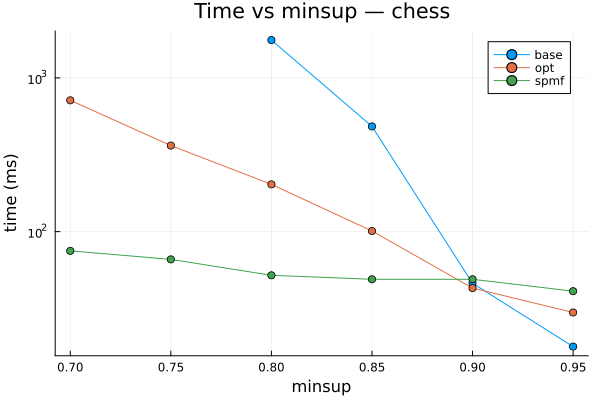
\includegraphics[width=0.85\linewidth]{../experiments/figures/time_chess.png}
    \caption{Thời gian chạy theo minsup trên Chess.}
    \label{fig:time-chess}
\end{figure}

Trên Chess, FP-Max trực tiếp (\texttt{opt}) thể hiện lợi thế rõ ở vùng output lớn. Tại minsup $0.80$, baseline naive-maximal mất 1762.92 ms trong khi \texttt{opt} chỉ mất 203.07 ms, nhanh hơn khoảng 8.68 lần; ở các ngưỡng thấp hơn ($0.75$, $0.70$) baseline bị skip vì mine-all bùng nổ, còn \texttt{opt} vẫn chạy (714.94 ms ở minsup $0.70$ với 891 tối đại). Khi minsup rất cao như $0.95$, output chỉ còn 11 tối đại nên chi phí cố định chiếm ưu thế và baseline lại nhanh hơn đôi chút (17.88 ms so với 29.81 ms). So với SPMF, \texttt{opt} vẫn chậm hơn (203.07 ms so với 52 ms ở minsup $0.80$), phản ánh khoảng cách giữa cài đặt học thuật và thư viện Java đã tối ưu lâu dài.

\begin{figure}[H]
    \centering
    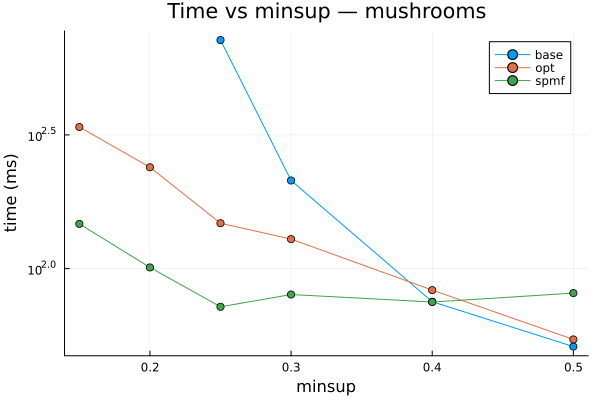
\includegraphics[width=0.85\linewidth]{../experiments/figures/time_mushrooms.png}
    \caption{Thời gian chạy theo minsup trên Mushrooms.}
    \label{fig:time-mushrooms}
\end{figure}

Hình \ref{fig:time-mushrooms} thể hiện xu hướng tương tự trên Mushrooms. Tại minsup $0.25$, \texttt{opt} nhanh hơn baseline khoảng 4.84 lần (147.81 ms so với 715.35 ms); ở minsup $0.30$ tỉ lệ thu hẹp còn 1.66 lần. Ở các ngưỡng cao ($0.4$, $0.5$) khi output nhỏ, hai bản xấp xỉ nhau và chi phí dựng cây cùng JIT chi phối.

\begin{figure}[H]
    \centering
    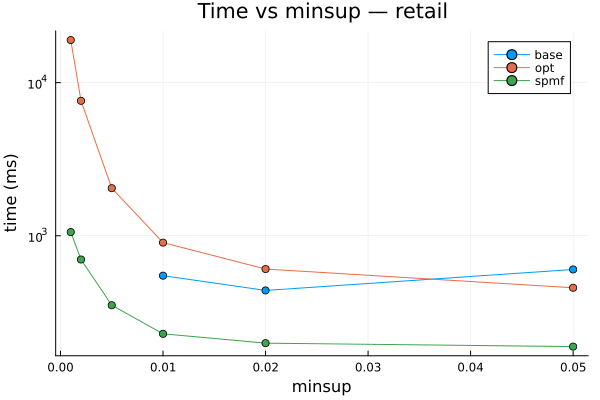
\includegraphics[width=0.85\linewidth]{../experiments/figures/time_retail.png}
    \caption{Thời gian chạy theo minsup trên Retail.}
    \label{fig:time-retail}
\end{figure}

Hình \ref{fig:time-retail} cho thấy một bức tranh ngược lại trên dữ liệu thưa. Vì Retail thưa, số tập phổ biến không lớn hơn số tối đại bao nhiêu nên phép tỉa của FP-Max ít có tác dụng, trong khi chi phí cài đặt --- node dạng \texttt{String} và bước tính lại support cho từng MFI trên toàn cơ sở dữ liệu --- lại lấn át. Tại minsup $0.01$, \texttt{opt} chậm hơn baseline (902.09 ms so với 548.92 ms). Ở minsup $0.001$, \texttt{opt} mất 18959.89 ms còn SPMF chỉ 1057 ms. Đây là điểm yếu rõ nhất của cài đặt FP-Max hiện tại và là động lực cho hướng tối ưu ở cuối mục.

\begin{figure}[H]
    \centering
    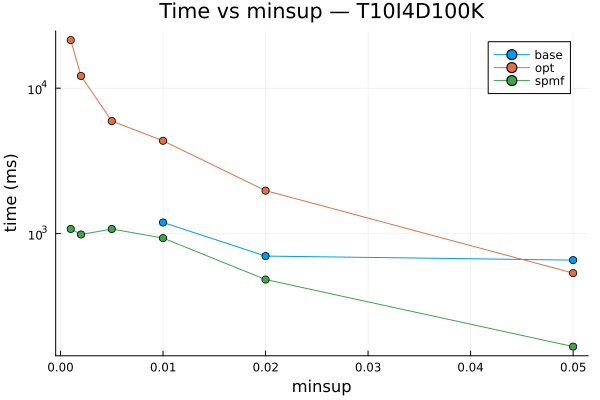
\includegraphics[width=0.85\linewidth]{../experiments/figures/time_T10I4D100K.png}
    \caption{Thời gian chạy theo minsup trên T10I4D100K.}
    \label{fig:time-t10}
\end{figure}

Trên T10I4D100K, vốn thưa và tổng hợp, xu hướng giống Retail: baseline nhanh hơn \texttt{opt} ở các điểm cả hai còn chạy (ví dụ minsup $0.01$: 1192.31 ms so với 4347.90 ms). Lợi ích nén tiền tố và tỉa siêu tập không đủ bù chi phí cài đặt trên dữ liệu thưa.

\begin{figure}[H]
    \centering
    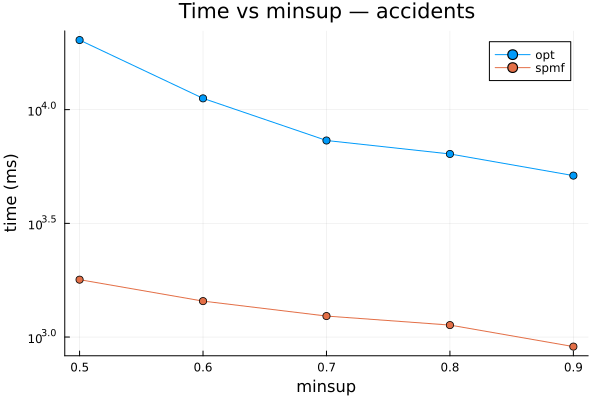
\includegraphics[width=0.85\linewidth]{../experiments/figures/time_accidents.png}
    \caption{Thời gian chạy theo minsup trên Accidents.}
    \label{fig:time-accidents}
\end{figure}

Hình \ref{fig:time-accidents} trình bày kết quả trên Accidents. Baseline bị bỏ qua hoàn toàn vì dữ liệu vừa lớn vừa dày khiến mine-all không khả thi --- đúng vùng mà FP-Max trực tiếp phát huy giá trị. \texttt{opt} chạy được ở mọi ngưỡng từ $0.9$ đến $0.5$, với thời gian từ 5.13 giây (minsup $0.9$, 1 tối đại) đến 20.23 giây (minsup $0.5$, 216 tối đại), chậm hơn SPMF khoảng 4--11 lần. Điểm yếu chính vẫn là cài đặt cấp phát nhiều object \texttt{String} cho conditional trees và tính lại support cho từng MFI.

\subsection{Số lượng tập tối đại theo minsup}

Hình \ref{fig:count-chess} và Hình \ref{fig:count-retail} minh hoạ quan hệ giữa minsup và số tập tối đại đầu ra. Chess tăng từ 11 tối đại ở minsup $0.95$ lên 891 tối đại ở minsup $0.70$. Retail tăng từ 4 tối đại ở minsup $0.05$ lên 3,452 tối đại ở minsup $0.001$.

\begin{figure}[H]
    \centering
    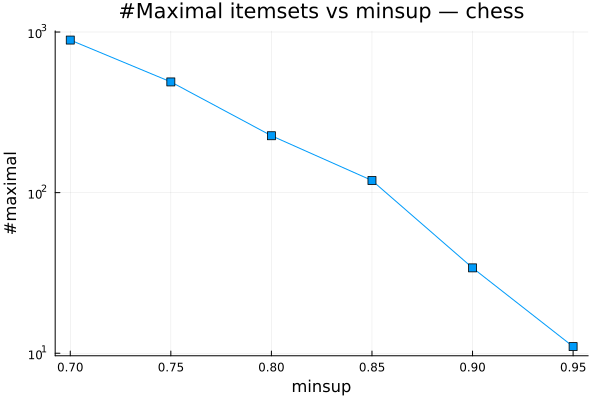
\includegraphics[width=0.82\linewidth]{../experiments/figures/count_chess.png}
    \caption{Số tập tối đại theo minsup trên Chess.}
    \label{fig:count-chess}
\end{figure}

\begin{figure}[H]
    \centering
    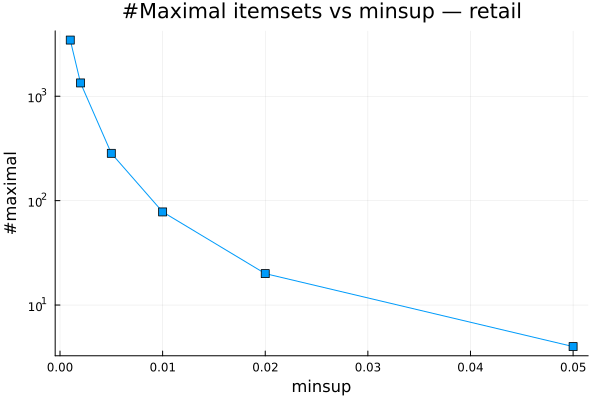
\includegraphics[width=0.82\linewidth]{../experiments/figures/count_retail.png}
    \caption{Số tập tối đại theo minsup trên Retail.}
    \label{fig:count-retail}
\end{figure}

Sự khác biệt giữa hai hình cho thấy độ dày dữ liệu ảnh hưởng mạnh đến output size. Chess có giao dịch dài và nhiều item đồng xuất hiện nên khi minsup giảm trong một khoảng hẹp, số tối đại tăng nhanh. Retail có nhiều item phân biệt nhưng giao dịch ngắn, vì vậy số tối đại chỉ tăng mạnh ở vùng minsup rất thấp. Đáng chú ý là số tập tối đại nhỏ hơn nhiều số tập phổ biến tương ứng: đây chính là lợi ích biểu diễn cô đọng mà FP-Max khai thác, và là lý do cài đặt trực tiếp khả thi trên Accidents trong khi baseline thì không.

\subsection{Bộ nhớ}

Hình \ref{fig:memory} so sánh lượng byte cấp phát giữa baseline và FP-Max tại một minsup trung bình của từng dataset. Trên dữ liệu dày, FP-Max cấp phát ít hơn hẳn: Chess ở minsup $0.85$ giảm từ 119.71 MB (base) xuống 25.23 MB (opt), khoảng 4.75 lần; Mushrooms ở minsup $0.30$ giảm từ 123.79 MB xuống 45.67 MB, khoảng 2.71 lần. Ngược lại, trên dữ liệu thưa FP-Max cấp phát nhiều hơn baseline: Retail ở minsup $0.02$ là 188.38 MB so với 116.27 MB, và T10I4D100K ở minsup $0.02$ là 434.60 MB so với 284.74 MB. Điều này nhất quán với phân tích thời gian: phép tỉa chỉ tiết kiệm khi có nhiều tập phổ biến không tối đại để cắt.

\begin{figure}[H]
    \centering
    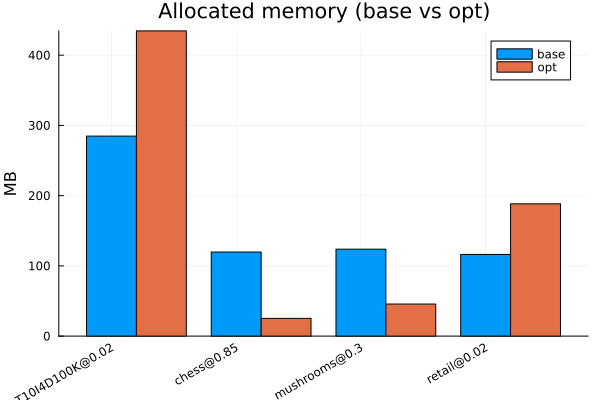
\includegraphics[width=0.85\linewidth]{../experiments/figures/memory.png}
    \caption{Bộ nhớ cấp phát của baseline naive-maximal và FP-Max tại minsup trung bình.}
    \label{fig:memory}
\end{figure}

Cột \texttt{alloc\_bytes} phản ánh tổng lượng cấp phát trong Julia, tức áp lực lên bộ thu gom rác (GC), chứ không phải dung lượng thường trú lớn nhất của tiến trình. Để đo trực tiếp peak memory thật, nhóm bổ sung một thực nghiệm riêng (\texttt{experiments/measure\_memory.jl}): mỗi cấu hình được chạy trong một tiến trình Julia độc lập rồi đọc \texttt{Sys.maxrss()} --- đỉnh resident set size (RSS) của tiến trình. Vì mỗi tiến trình mới reset RSS, giá trị \texttt{maxrss} cuối là peak của đúng lần chạy đó. Hàng \emph{sàn} chỉ load package và dữ liệu mà không mining, cho biết phần RSS do runtime Julia chiếm. Bảng \ref{tab:peak-rss} tổng hợp kết quả.

\begin{table}[H]
    \centering
    \caption{Peak RSS thật (\texttt{Sys.maxrss}) đo trong tiến trình riêng cho mỗi lần chạy. Cột \emph{sàn} là cấu hình chỉ load dữ liệu, không mining.}
    \label{tab:peak-rss}
    \begin{tabular}{l r r r r}
        \toprule
        Dataset & minsup & Sàn (MB) & base peak (MB) & opt peak (MB) \\
        \midrule
        Chess      & 0.80 & 403.83 & 456.60 & 441.97 \\
        Chess      & 0.85 & 403.83 & 437.32 & 441.92 \\
        Mushrooms  & 0.30 & 420.38 & 449.15 & 448.55 \\
        Retail     & 0.01 & 463.50 & 500.04 & 534.55 \\
        T10I4D100K & 0.01 & 461.41 & 791.33 & 842.44 \\
        \bottomrule
    \end{tabular}
\end{table}

Bảng \ref{tab:peak-rss} cho thấy ba điểm. Thứ nhất, sàn RSS do runtime Julia, load package và dữ liệu chiếm khoảng $404$--$463$ MB, lớn hơn nhiều phần bộ nhớ làm việc của thuật toán, nên peak RSS tuyệt đối bị chi phối bởi sàn này. Thứ hai, trên dữ liệu dày FP-Max thường trú thấp hơn hoặc xấp xỉ baseline: Chess $0.80$ peak giảm từ $456.60$ MB (base) xuống $441.97$ MB (opt), nhất quán với xu hướng \texttt{alloc\_bytes}; còn trên dữ liệu thưa (Retail, T10I4D100K) FP-Max thường trú cao hơn, đúng với việc cấp phát nhiều hơn baseline ở vùng này. Thứ ba, peak RSS thật nhỏ hơn nhiều tổng \texttt{alloc\_bytes}, vì phần lớn cấp phát là tạm thời và bị GC thu hồi nên không cùng lúc thường trú. Hai chỉ số do đó bổ sung cho nhau: \texttt{alloc\_bytes} đo áp lực cấp phát/GC, còn peak RSS đo dung lượng thực tế của tiến trình.

\subsection{Khả năng mở rộng}

Hình \ref{fig:scalability} trình bày thực nghiệm scalability, lấy các prefix 10\%, 25\%, 50\%, 75\% và 100\% của Retail và Accidents. Với Accidents ở minsup $0.7$, FP-Max tăng từ 690.13 ms trên 34,018 giao dịch lên 7673.25 ms trên 340,183 giao dịch; khi số giao dịch tăng 10 lần, thời gian tăng khoảng 11.1 lần --- gần tuyến tính, hơi siêu tuyến do chi phí dựng và duyệt cây tăng theo độ sâu. Số tối đại dao động quanh 19--26 nên không chi phối xu hướng.

Với Retail ở minsup $0.01$, FP-Max tăng từ 81.51 ms trên 8,816 giao dịch lên 1120.50 ms trên 88,162 giao dịch. Baseline naive-maximal vẫn nhanh hơn FP-Max ở mọi kích thước Retail (ví dụ 27.13 ms so với 81.51 ms ở 10\%), một lần nữa khẳng định trên dữ liệu thưa chi phí cài đặt FP-Max vượt lợi ích tỉa.

\begin{figure}[H]
    \centering
    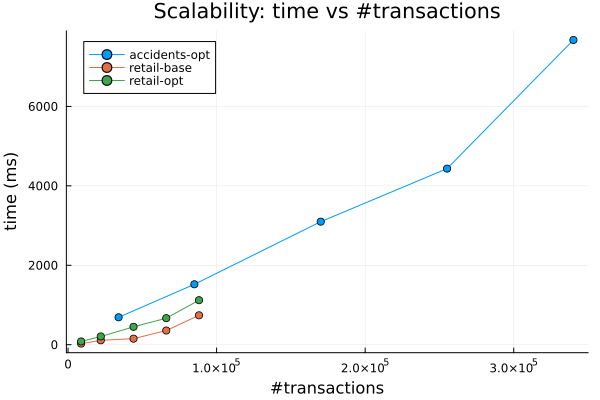
\includegraphics[width=0.88\linewidth]{../experiments/figures/scalability.png}
    \caption{Khả năng mở rộng theo số lượng giao dịch.}
    \label{fig:scalability}
\end{figure}

\subsection{Ảnh hưởng của độ dài giao dịch}

Thí nghiệm cuối dùng dữ liệu tổng hợp 20,000 giao dịch, 100 item, minsup $0.03$, và tăng độ dài giao dịch trung bình từ 5 đến 25. Bảng \ref{tab:txnlen} cho thấy thời gian tăng mạnh khi độ dài trung bình đạt 20 và 25.

\begin{table}[H]
    \centering
    \caption{Ảnh hưởng của độ dài giao dịch trung bình lên thời gian chạy FP-Max.}
    \label{tab:txnlen}
    \begin{tabular}{r r r}
        \toprule
        AvgLen & Time ms & \#Tối đại \\
        \midrule
        5 & 276.31 & 100 \\
        10 & 636.31 & 100 \\
        15 & 1349.64 & 100 \\
        20 & 19213.50 & 4,950 \\
        25 & 30039.70 & 4,950 \\
        \bottomrule
    \end{tabular}
\end{table}

\begin{figure}[H]
    \centering
    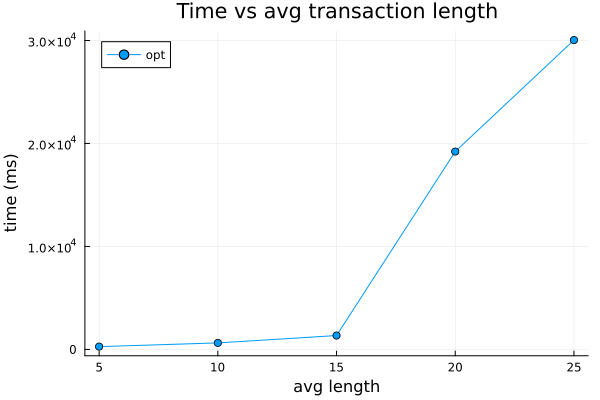
\includegraphics[width=0.82\linewidth]{../experiments/figures/txnlen.png}
    \caption{Thời gian chạy FP-Max khi tăng độ dài giao dịch trung bình.}
    \label{fig:txnlen}
\end{figure}

Kết quả này phù hợp với lý thuyết: giao dịch dài làm tăng xác suất các item cùng xuất hiện, làm FP-tree dày hơn và số tập tối đại tăng. Khi output size nhảy từ 100 lên 4,950 tối đại (giữa độ dài 15 và 20), thời gian cũng nhảy từ 1349.64 ms lên 19213.50 ms, tức tăng theo bậc lớn hơn nhiều so với mức tăng tuyến tính của độ dài giao dịch; Hình \ref{fig:txnlen} minh hoạ rõ bước nhảy này, đúng với cận mũ ở trường hợp xấu khi số tối đại $M$ bùng nổ.

\subsection{Nhận xét và hướng tối ưu tiếp theo}

Thực nghiệm cho thấy cài đặt FP-Max của nhóm đúng so với SPMF FPMax trên mọi cấu hình kiểm tra. Điểm mạnh quyết định là FP-Max trực tiếp hoàn tất trong những vùng mà baseline naive-maximal không khả thi --- toàn bộ Accidents và các ngưỡng thấp trên dữ liệu dày --- nhờ chỉ giữ biểu diễn tối đại và tỉa theo siêu tập. Trên dữ liệu dày như Chess và Mushrooms ở minsup thấp, FP-Max nhanh hơn baseline nhiều lần và cấp phát ít hơn rõ rệt.

Điểm yếu có hai mức. So với baseline, FP-Max chậm hơn trên dữ liệu thưa (Retail, T10I4D100K) vì phép tỉa ít tác dụng còn chi phí cài đặt cao. So với SPMF, FP-Max chậm hơn trên hầu hết cấu hình lớn. Nguyên nhân chính nằm ở cài đặt: FP-Max hiện dùng FP-tree với node \texttt{String} và tính lại support cho từng MFI bằng một lần quét toàn cơ sở dữ liệu.

Từ đó, hai hướng tối ưu cụ thể có thể làm tiếp. Thứ nhất, chuyển FP-Max sang dùng cấu trúc cây mã hoá số nguyên như \texttt{FPGrowthOpt} (header và children typed, \texttt{@inbounds}) để loại chi phí \texttt{String} trong hot loop. Thứ hai, mang support theo trong quá trình khai thác để bỏ hẳn bước tính lại support cho từng MFI ở cuối, vốn tốn một lần quét dữ liệu mỗi tối đại. Ngoài ra, có thể thay danh sách MFI tuyến tính bằng một MFI-tree để phép kiểm tra siêu tập có chi phí dưới tuyến tính, và song song hoá các nhánh conditional tree độc lập.
